\chapter{Software Packages used in this work}
\label{cha:software}

This chapter illustrates the main software tools used in this work. First, the \acrfull{mbdyn}  is shortly presented in Section \ref{sec:mbdyn}. Then, the coupling library \acrfull{precice} is introduced in Section~\ref{sec:precice}.


\section{MBDyn}
\label{sec:mbdyn}


\acrshort{mbdyn} is free and open-source\footnote{the software is available through a public git repository \href{https://gitlab.polimi.it/Pub/mbdyn}{gitlab.polimi.it/Pub/mbdyn}} general purpose Multibody Dynamics analysis software developed at the \textit{Dipartimento di Scienze e Tecnologie Aerospaziali}  of the University Politecnico di Milano.

Most of the information concerning MBDyn is taken from the official documentation given in the software website\footnote{MBDyn website: \href{https://www.mbdyn.org/}{mbdyn.org}} and from the input manual\footnote{a copy can be found at the following link [\href{https://www.mbdyn.org/userfiles/documents/mbdyn-input-1.7.3.pdf}{input manual}] or in the code repository}.

MBDyn allows to build a system to simulate multi-body dynamics, which\footnote{see Wikipedia entry: \href{https://en.wikipedia.org/wiki/Multibody_system}{Multibody system}} is the study of the behavior of interconnected rigid or flexible bodies, each of which may undergo large translational and rotational displacements.

MBDyn can simulate linear and non-linear dynamics of rigid and flexible bodies (including geometrically exact and composite-ready beam and shell finite elements, component mode synthesis elements, lumped elements) subjected to kinematic constraints, external forces and control subsystems\cite{masarati2014efficient}. 
MBDyn has been developed to serve as an analysis tool for rotorcraft research and can simulate essential fixed-wing and rotorcraft aerodynamics.

As explained more in detail later, MBDyn is open to be connected to other software components to perform multi-physics simulations. In particular, it is possible to pass externally computed forces and to steer the multi-body simulation from an external \acrshort{api}: this feature has been particularly useful in building and \textit{adapter} to couple MBDyn with the library preCICE (see Chapter \ref{cha:adapter}).

In this section we give a short introduction to some of the relevant features of MBDyn, starting form basic information on the input file syntax (Section \ref{sec:mbd-syntax}), and the output files (Section \ref{sec:mbd-output}). Then some of the elements relevant for the description of the models used in the this work are presented: nodes (Section \ref{sec:mbd-node}), beam elements (Section \ref{sec:mbd-beam}), bodies (Section \ref{sec:mbd-body}), joints (Section \ref{sec:mbd-joint}) and forces (Section \ref{sec:mbd-forces}). 


\subsection{Basic syntax}
\label{sec:mbd-syntax}

MBDyn is a command line tool and can be generally started from a terminal passing an input file containing all the information required to perform a simulation. 

The input files is structured in blocks and each block has a syntax described in Backus Naur form in the input manual.

\lstset{language=mbdyn}
\begin{lstlisting}[caption=MBDyn input file structure,label=lst:mbd-struct]
begin : data ;
    # select a problem
    problem : initial value ;
end : data ;

begin : initial value ;
    # problem-specific data
end : initial value ;

begin : control data ;
    # model control data
end : control data ;

begin : nodes ;
    # nodes data
end : nodes ;

begin : elements ;
    # elements data
end : elements ;
\end{lstlisting}

As illustrated in listing \ref{lst:mbd-struct}, statements are logically divided in blocks. Each block is opened by a \texttt{begin} statement and it is closed by an \texttt{end} statement.

The sequence of relevant valid blocks is:

\begin{itemize}
    \item \texttt{data}: it defines the kind of problem to be solved by the analysis. The most significant one is \texttt{initial value} and is already defined in the example. 
    \item type of problem:  it takes the name of the problem defined in the data block (\texttt{initial value} in this case) and contains all the information required by the integration method to perform the desired simulation (e.g. simulation type, time step, number of iterations, tolerance ...).
    \item \texttt{control data}: it mostly contains the required information to ensure that a consistent model will be generated (i.e. the number of nodes, elements, forces...).
    \item \texttt{nodes}: this block contains all the nodes required by the simulation. They are defined as the entities that make degrees of freedom available to the simulation, so they must exist before any element is generated.
    \item \texttt{elements}: it contains all the elements. They are defined as the entities that generate equations using the degrees of freedom provided by the nodes.
\end{itemize}

We focus now on the main entities of a MBDyn simulation, namely nodes and elements. A detailed example of the input file used in most simulations in this work can be found in Appendix \ref{sec:mbdyn-input-file}.


\subsection{Nodes}
\label{sec:mbd-node}

Nodes are the basic blocks of a model: they instantiate kinematic degrees of freedom and the corresponding equilibrium equations. There can be different type of nodes in MBDyn, we focus here on \texttt{structural nodes}.

Structural nodes can have 3 degrees of freedom, thus describing the kinematics of point mass motion in space  (position) or 6 DoFs (position and orientation), and thus describing the kinematics of rigid-body motion in space.

Each node has a unique label and can be specified in different ways:

\begin{itemize}
	\item \texttt{static}: this keyword instantiates only equilibrium equations (force for 3 DoF nodes or force and moment for 6 DoF nodes)
	\item \texttt{dynamic}: this also instantiates momentum (3 and 6 DoFs) and momenta moment (6~DoFs)
\end{itemize}

Also \texttt{modal} and \texttt{dummy} nodes exist, but are beyond the scope of this work. Nodes are the starting point to define the elements of a simulation.


\subsection{Elements}
\label{sec:mbd-elem}

Elements constitute the components of the multi-body model. Each has a unique numerical label and is connected to one or more nodes. They write contributions to nodes equations and represent \textit{connectivity} and \textit{constitutive properties}.

%Elements that require both displacement and orientation can only be connected to 6 DoFS nodes.

There exist many types of elements in MBDyn, we focus here on the ones used in the \acrshort{fsi} simulation: beams, bodies, joints and forces.



\subsection{Beam elements}
\label{sec:mbd-beam}

As briefly introduced in Section \ref{sec:beam}, when simulations involve slender bodies, it is particularly interesting to use a 1D finite element model together with a form of mapping between the interface (wet surface) and the model to exchange kinematics and dynamics information. This can be performed in MBDyn using \texttt{beam} elements (described in this section) and the \texttt{external structural mapping} element (described in Section \ref{sec:mbd-forces}).

MBDyn models slender deformable components by means of finite volume \texttt{beam} elements with a high level of flexibility.

The beam element is defined by its nodes and a reference line; although 2 and 3 nodes beam elements are implemented, only \texttt{beam3} are considered here (Figure \ref{fig:mbdyn-beam-model}). Each node of the beam is related to a \texttt{structural node} (node 1 to 3 in Figure \ref{fig:mbdyn-beam-model}) by an offset ($o_1$ to $o_3$) and a relative orientation.

\begin{figure}[htbp!]
	\centering
	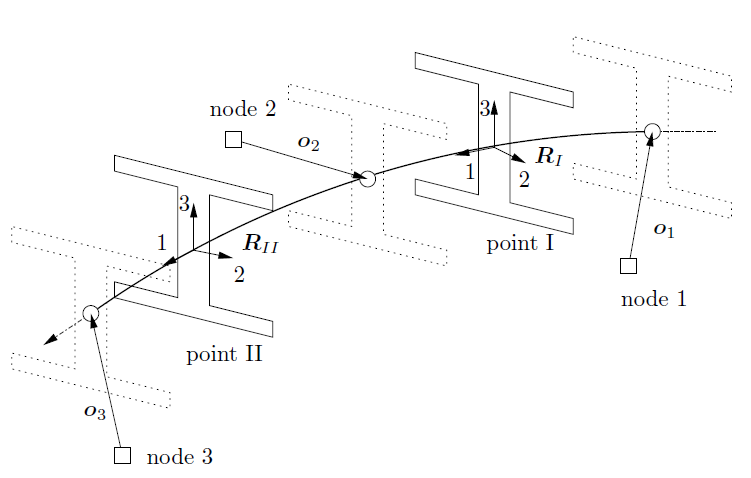
\includegraphics[width=0.8\textwidth]{images/beam_model}
	\caption{MBDyn beam model, taken from the input manual}
	\label{fig:mbdyn-beam-model}
\end{figure}


The Finite Volume approach described in \cite{ghiringhelli2000multibody} is used to model the beam element. It computes the internal forces as functions of the reference line strain and as functions of the  orientation at the \textit{evaluation points} (i.e. integration points, point I and II in Figure \ref{fig:mbdyn-beam-model}) that are between nodes 1 and 2, and between nodes 2 and 3 (at $\xi =-1/\sqrt{3}$ and $\xi = 1/\sqrt{3}$ of a non-dimensional abscissa $-1\leq \xi \leq 1$ ranging from node 1 to node 3).


A 6D constitutive law is defined at each evaluation point: it relates the strains and the curvatures of the beam (and their time derivatives) to the internal forces and moments at the evaluation points in the form:

\begin{equation}
	\begin{Bmatrix}
		F_x \\ F_y \\ F_z \\ M_x \\ M_y \\ M_z
	\end{Bmatrix} = f
	\begin{pmatrix}
		\begin{Bmatrix}
			\epsilon_x \\ \gamma_y \\ \gamma_z \\ \kappa_x \\ \kappa_y \\ \kappa_z
		\end{Bmatrix} , 
		\begin{Bmatrix}
			\dot{\epsilon_x} \\ \dot{\gamma_y} \\ \dot{\gamma_z} \\ \dot{\kappa_x} \\ \dot{\kappa_y} \\ \dot{\kappa_z}
		\end{Bmatrix}
	\end{pmatrix}
\end{equation}


Using the convention of \textit{x-axis} as beam axis we have:

\begin{itemize}
	\item $F_x$: axial force component,
	\item $F_y$ and $F_z$: shear force components,
	\item $M_x$: torsional moment component,
	\item $M_y$ and $M_z$: bending moment components,
	\item $\epsilon_x$: axial strain component,
	\item $\gamma_y$ and $\gamma_z$: shear strain components,
	\item $\kappa_x$: torsional curvature component,
	\item $\kappa_y$ and $\kappa_z$: bending curvature components,
	\item $f$: constitutive law.
\end{itemize}


\subsubsection{Beam section Constitutive Law}

In dynamic simulations, linear elastic or viscoelastic laws are generally used, even though nonlinear laws can be used.  Focusing on linear laws, MBDyn allows the user to define every kind of constitutive laws, going from an isotropic beam section to a fully anisotropic one: in fact the entire $6 \times 6$ constitutive matrix can be provided. It is up to the user to define a valid law as the matrix must satisfy some constraints, e.g. it must be symmetric. The simplest case of linear elastic constitutive law is represented in Equation \ref{eq:iso-const}, in which a diagonal matrix relates internal forces to strain and curvature of the beam. 

\begin{equation}
    f = \begin{bmatrix} EA & 0 & & \ldots &  & 0 \\
                          & \chi GA &  & & & &  \\
                          & & \chi GA & & & \\
                          & & & GJ_p & & \vdots \\
                          & &  sym. & & EJ_y & 0 \\
                          & & & & & EJ_z
    \end{bmatrix} \cdot 
    \begin{Bmatrix}
		\epsilon_x \\ \gamma_y \\ \gamma_z \\ \kappa_x \\ \kappa_y \\ \kappa_z
	\end{Bmatrix}
    \label{eq:iso-const}
\end{equation}

The simplest case of linear viscoelastic law uses a proportional factor to be applied to the stiffness matrix of Equation \ref{eq:iso-const} such that: $viscosity=factor \cdot stiffness$.






In the context of FSI simulations, this feature allows the user to define a section constitutive law that is independent from the shape of the beam itself. Thus the aerodynamic aspects and the structural aspects are handled by two distinct elements of the model: i.e. the interface mesh defines the aerodynamic forces and the beam constitutive law defines the structural properties.   

Some studies about the definition of general beam section constitutive properties (\textit{composite beam section characterization}) are available in the literature: an early work can be found in \cite{giavotto1983anisotropic}, a review in \cite{hodges1990review} or an application to wind turbine blades in \cite{kim2013development}.


\subsection{Bodies}
\label{sec:mbd-body}

The \texttt{body} element describes a lumped rigid body when connected to a regular, 6 DoF structural node, or a point mass when connected to a rotationless, 3 DoF structural node. It can be used in connection with a structural element to give inertial properties: for example, in a \texttt{beam} element (see Section \ref{sec:mbd-beam}), 2 bodies are added to the evaluation points of the beam to account for lumped inertia of each portion in which the beam is divided. 


\subsection{Joints}
\label{sec:mbd-joint}

\texttt{structural} nodes can be constrained by means of \texttt{joint} elements. Many different joints are available. In the FSI model the following types of joints are used:

\begin{itemize}
	\item \texttt{clamp}: grounds all 6 DoFs of a node in an arbitrary position and orientation.
	\item \texttt{total joint}: allows to arbitrarily constrain specific components of the relative position and orientation of two nodes\cite{masarati2013formulation}.
\end{itemize}


\subsection{Forces}
\label{sec:mbd-forces}

The \texttt{force} element is a general means to introduce a right-hand side term to the equations. Structural forces are specific to structural
nodes and  have three components that may depend on arbitrary parameters and a location in space.

MBDyn allows to communicate with an external software that computes forces based on information regarding the kinematics of the model. This feature is at the basis of the development of the \textit{adapter}. The following elements can be used.


\subsubsection{External Structural}

The \texttt{External Structural} element allows to communicate with an external software that computes forces applied to a pool of \texttt{nodes} and may depend on the kinematics of those nodes. In this case forces are applied directly to the nodes. In a FSI model, this would require that each interface mesh node has a correspondent MBDyn structural node. 

\subsubsection{External structural mapping}


This element is similar to the previous one, but the nodes where forces are applied and the kinematics is computed depend on structural nodes through a linear mapping. This element has been used in building the adapter. In order to use the \texttt{external structural mapping} elements, the following steps have to be performed:

\begin{enumerate}
	\item a set of points is defined for each \texttt{structural node} according to a specified offset. Those points are used to compute the kinematics of the interface points, originating from the rigid-body motion of the structural nodes,
	\item before the simulation, a linear mapping matrix $H$ is generated starting from the position of the above points and the interface mesh points (this is performed by means of an \texttt{Octave} script which is part of MBDyn). The matrix is stored in sparse form,
	\item the mapping matrix is used during the simulation to map forces and kinematics between the interface nodes and the structural nodes.
\end{enumerate}

The constant matrix mapping allows to compute the position and the velocity of the \textit{interface} points as function of the points rigidly offset from structural nodes:

\begin{subequations}
	\begin{eqnarray}
		x_{interf} &=& H x_{mbdyn} \\
		\dot{x}_{interf} &=& H \dot{x}_{mbdyn} 
	\end{eqnarray}
\end{subequations}

The same matrix is used to map back the forces onto structural nodes based on the preservation of the work done in the two domains:

\begin{equation}
	\delta x_{mbdyn}^T \cdot f_{mbdyn} =  \delta x_{interf}^T \cdot f_{interf} = \delta x_{mbdyn}^T \cdot H^T \cdot f_{interf} 
\end{equation}

which implies

\begin{equation}
	f_{mbdyn} = H^T f_{interf}
\end{equation}

When performing an \acrshort{fsi} simulation with strong coupling (see Section \ref{sec:strong-coupling}), MBDyn may need to compute multiple iterations of the same time step in order to reach global convergence. This is performed by using the keyword \texttt{tight} in the coupling of the \texttt{external structural mapping}. The computation and the communication pattern is the following:

\begin{enumerate}
	\item MBDyn sends the predicted kinematics for time step $k$,
	\item MBDyn receives a set of forces sent by the external peer; those forces are computed based on the kinematics at iteration $j$,
	\item MBDyn continues iterating until convergence using the last set of forces until, while reading the forces, it is informed that the external peer converged. this implies that MBDyn solves the kinematics for time step $k$ at iteration $j$ using the forces evaluated by the external solver for iteration $j-1$ .
\end{enumerate}

The communication with the external software, in our case the adapter itself, is performed by means of a local unix socket.


\subsection{Simulation output}
\label{sec:mbd-output}

There are different output files regarding a simulation performed with MBDyn. the name of those files is specified with the option \texttt{-o} (otherwise the name is the same as the input file) and the extensions are:

\begin{itemize}
    \item \texttt{.out}: for miscellaneous output
    \item \texttt{.mov}: for kinematic output of the nodes
    \item \texttt{.ine}: for the dynamic output of the nodes
    \item \texttt{.frc}: for the output of force elements
    \item \texttt{.act}: for the output of beam elements
    \item \texttt{.jnt}: for the output of joint elements
\end{itemize}

The \texttt{.out} file contains information regarding the simulation iterations residuals while other files are described in more detail in Appendix \ref{sec:mbdyn-output-file}.



%
%output
%
%If we copy the above written code to a file called, say, “rigidbody”, and invoke
%mbdyn -f rigidbody
%after a while we obtain the results of the simulation in a set of files called “rigidbody.<ext>”.
%In this case, the extensions will be:
%• out for miscellaneous output
%• mov for the kinematic output of the node
%• ine for the dynamic output of the node
%• frc for the output of the force
%The first file (out) will be ignored at present. The second file (mov) will contain Nnodes
%by Ntimesteps lines formatted as:
%• the node label
%• the three coordinates of the position of the node
%• the three Euler-like angles that define the orientation of the node (following the
%1, 2, 3 convention)
%• the three components of the velocity of the node
%• the three components of the angular velocity of the node
%all the above mentioned quantities are expressed in the global inertial frame
%



\section{preCICE}
\label{sec:precice}

The main information concerning \acrshort{precice} is taken from the official documentation: i.e. \cite{gatzhammer2014efficient} and  \cite{bungartz2016precice}. The preCICE website is also a source of documentation\footnote{\href{http://www.precice.org}{www.precice.org}}.

The open-source\footnote{The code can be accessed via Github: \href{https://github.com/precice/precice}{github.com/precice/precice}} software library preCICE provides the components to connect traditional single-physics solvers and create a partitioned multi-physics simulation (e.g. fluid-structure interaction, conjugated heat transfer, solid-solid interaction, etc.).
It aims at coupling existing solvers in a partitioned black-box manner (see Section \ref{sec:coupling}):  only minimal information about the solver is available and connection involves just the interface nodes. 

In order to be flexible and easily implemented, the impact on the solvers should be as minimal as possible: for this reason, preCICE offers a high level \acrfull{api} (Section \ref{sec:pc-api}) in different languages, such as C/C++, Fortran and Python.
The ability to switch among different solvers is advantageous as it provides a lot of flexibility in developing and testing new coupled components.

In a nutshell, preCICE simply affects the input and observes the output of the solvers (called \textit{participants}). The required data and control elements are accessed using an \textit{adapter}, i.e. a  ``glue code'' that is attached to the corresponding solver and communicates the information with the library.

\acrshort{precice} makes all the actions required to perform a coupled simulation: 

\begin{itemize}
	\item it implements the coupling strategy (Section \ref{sec:pc-coupling}),
	\item it verifies convergence criteria (Section \ref{sec:pc-coupling}),
	\item it instantiates the communication between the participants (Section \ref{sec:pc-comm}) ,
	\item it computes the mapping of data between meshes (Section \ref{sec:pc-map}). 
\end{itemize}

preCICE is configured by means of an \acrfull{xml} file (Section \ref{sec:pc-config}).



\subsection{Implemented coupling strategies}
\label{sec:pc-coupling}

The \textit{partitioned approach} (Section \ref{sec:coupling}) is obviously the coupling strategy adopted by preCICE. It allows both \textit{explicit} (Section \ref{subsec:explicit}) and \textit{implicit} coupling (Section \ref{subsec:implicit}). The possible variants are four:

\begin{itemize}
	\item \texttt{serial-explicit}: a serial, weakly coupled algorithm (Figure \ref{fig:serial-explicit}). The first solver uses the second solver solution at the last time step to compute its current solution. In contrast, the second solver needs the current first solution to compute its solution at the same time instance. The order of execution is user defined.
	\item \texttt{parallel-explicit}: both solvers advance in parallel (Figure \ref{fig:parallel-explicit}) and exchange data at the end of each time step, resulting in a less stable procedure. The bottleneck of this procedure is related to the most time consuming solver.
	\item \texttt{serial-implicit}: a serial strongly coupled algorithm (Figure \ref{fig:serial-implicit}). The user can define the order of execution, the coupling algorithm (basically all the algorithms described in Section \ref{sec:strong-coupling}) and its parameters in a section of the configuration file named \texttt{acceleration}.
	\item \texttt{parallel-implicit}: again both solvers execute in parallel (Figure \ref{fig:parallel-implicit}). An implicit scheme modifies the result of the fixed-point iteration on both data \cite{mehl2016parallel}. 
\end{itemize}



\subsection{Communication strategies}
\label{sec:pc-comm}

All the participants need to communicate with each other, in order to share coupling data.
Each solver might be executed in multiple processes or on different nodes of a cluster (\textit{intrafield parallelism}).
This form of parallelization requires efficient forms of communication between the solver in order to avoid that data transfer becomes a bottleneck during a simulation.

preCICE implements a fully parallel process-to-process communication approach \cite{Shukaev2015} using:

\begin{itemize}
	\item \textit{\acrfull{mpi}}: available on 	most scientific computers, it may be necessary to adapt/change the MPI versions of the respective single-physics solvers or of preCICE.
	\item \textit{\acrfull{tcpip}}: popular means of network communication and free of incompatibilities between versions.
\end{itemize}

As to performances, \acrshort{mpi} is the best technique especially when a high numbers of nodes is present. Anyway, socket communication is quite as fast, such that
both techniques are very well-suited for larger-scale simulations \cite{gatzhammer2014efficient}.

In each solver, executed in parallel, one ``master'' process is defined to manage the progress of the simulation. No central node is required. The participating
processes use asynchronous point-to-point (M:N) communication. The channels are static and defined in the beginning of the simulation. This sets a limit in using preCICE with dynamically adaptive meshes or immersed boundaries.

\subsection{Data mapping}
\label{sec:pc-map}

Even if volume coupling is possible, preCICE is mainly designed to couple simulations that share a common surface boundary (namely \textit{conforming meshes}, in the terminology used in Section~\ref{sec:conforming-mesh}). The meshes do not need to be node-to-node coincident, so it is necessary to map variables at the interface, preserving the geometry (i.e. no gaps or superpositions at the interface) and the mass and energy balances. 

The user defines which data are shared by each \textit{participant} (i.e. solver) and the way data is shared in the configuration section named \texttt{mapping}. As described in Section~\ref{sec:data-mapping}, two kinds of mapping are available:

\begin{itemize}
	\item \texttt{consistent}: the value of a node at the one grid is the same as the value of the corresponding node (or nodes) at the other grid. In general the number of fluid nodes is at least the same or, more often, exceeds the nodes of the structure, so a single structural node is associated to several fluid nodes. The mapping of displacements is consistent: in the simplest case, all fluid nodes experience the same displacement of a single solid node, otherwise an interpolation is performed (see Section~\ref{sec:data-mapping} for a detailed explanation and Figure~\ref{fig:consistent} for an example).
	\item \texttt{conservative}: in the same conditions as before, forces are mapped from multiple fluid nodes to a single solid node in an additive manner (see Section~\ref{sec:data-mapping} and Figure~\ref{fig:conservative} for an example).
\end{itemize} 

Along with the mapping strategy, a method must be defined: \texttt{nearest-neighbor}, \texttt{nearest-projection}, \texttt{rbf} (see Section \ref{sec:data-mapping}). For the latest method, preCICE implements a wide variety of basis functions, with Gaussian and thin plate splines being the most widely used.

 

\subsection{Configuration}
\label{sec:pc-config}

In order to run a multi-physics simulation with preCICE, all the participating, \textit{adapted} solvers have to be started (the order is irrelevant).
Some configuration files are needed:

\begin{itemize}
	\item each adapter generally needs its own configuration file. It normally contains information about the boundaries (wet-surface) used for the coupling, the names of exchanged data, mesh and the name of the common preCICE configuration file, together with other parameters, specific to the adapter. The one for the MBDyn adapter will be described in more detail in Chapter \ref{cha:adapter} and in Appendix \ref{app:mbd-config-file}.
	\item preCICE configuration file: This is an \acrshort{xml} file and each participant points at it. It defines all the information relevant to the simulation:
	\begin{itemize}
		\item type and name of exchanged data and meshes over which those data are passed,
		\item which solvers participate in the simulation, which data produce or consume, and how the mapping is performed,
		\item how solvers communicate among each other,
		\item the coupling scheme and all the concerning necessary information. 
	\end{itemize}
	
The structure of a preCICE configuration file is illustrated in Appendix \ref{app:pc-config-file}.
		
\end{itemize}


\subsection{Application Program Interface}
\label{sec:pc-api}

A solver, in order to be coupled to preCICE, must either provide a way to access its core functions (e.g. initialize, set input data, read output, advance...) from outside the code (via API, socket, etc...) or it has to be slightly modified in order to perform all the operations required by the preCICE library.

The result is an \textit{adapter}, which can be the modified and recompiled original solver, or a standalone piece of code that communicates with the original unmodified solver on one side and with the preCICE library on the other. The adapter groups together all the calls to the preCICE methods from its API (a list of the API calls, taken from the official documentation, can be found in Appendix \ref{sec:api-code}).

While preCICE is written in C++, there exist APIs also for other languages, so that the adapter can be written also in C, Fortran or Python.

A coupling consists of a configuration and an initialization phase, multiple coupling advancements and a finalization phase: the general structure of an adapter can be found in Appendix~\ref{sec:adapter-code}.


\subsection{Official Adapters}
\label{sec:pc-adapters}


This work introduces an adapter to preCICE for MBDyn. It is based on previous MBDyn adapters and on the examples given on the preCICE website\footnote{\href{https://github.com/precice/precice/wiki/Adapter-Example}{github.com/precice/precice/wiki/Adapter-Example}}.
Official adapters are currently available for several free solvers, e.g. CalculiX, Code-Aster and SU2. Also some closed-source software packages are supported. A (maybe outdated) list of official adapters can be found in \cite{uekermann2017official}, while the current status of coupled codes can be found at the following link: \href{https://www.precice.org/codes/}{preCICE adapters}.


